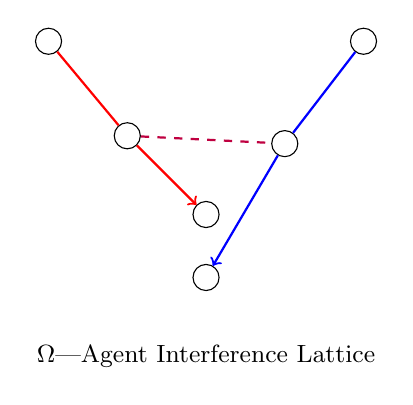
\begin{tikzpicture}[
    agent/.style={circle, fill=white, draw=black, minimum size=5pt},
    traj/.style={->, thick}
]

\node[agent] (A1) at (-2,1) {};
\node[agent] (A2) at (-1,-0.2) {};
\node[agent] (A3) at (0,-1.2) {};

\node[agent] (B1) at (2,1) {};
\node[agent] (B2) at (1,-0.3) {};
\node[agent] (B3) at (0,-2) {};

\draw[traj, red] (A1)--(A2)--(A3);
\draw[traj, blue] (B1)--(B2)--(B3);

\draw[dashed, thick, purple] (A2) -- (B2);

\node at (0,-3) {\small $\Omega$---Agent Interference Lattice};

\end{tikzpicture}